\section{Results}
We gathered a good baseline of data for 80MHz vs 40MHz performance in
both indoor and outdoor environments. Unfortunately, as detailed in
\ref{sec:methodology} we were unable to coherently measure the
performance of different MCS settings. Additionally, we ran out of
time to gather intentionally non-beamformed data for all of the
clients. \todo{discuss what}

All graphs in this section are generated from packet captures
performed by the \texttt{iperf} client unless otherwise noted. Error
bars denote a single standard deviation from the mean.

\subsection{Signal Strength}
We were, however, able to measure beamformed signal strength over
distance and through objects with 80MHz vs 40MHz quite effectively
with both the Intel 7260 and the Macbook. Unfortunately the Surface
was unable to provide radiotap headers during capture, so we have no
information about its recieved signal strength.

\tabcolsep=0.11cm



\subsubsection{Outdoor Clean Testing}

\begin{figure}[!h]
\centering
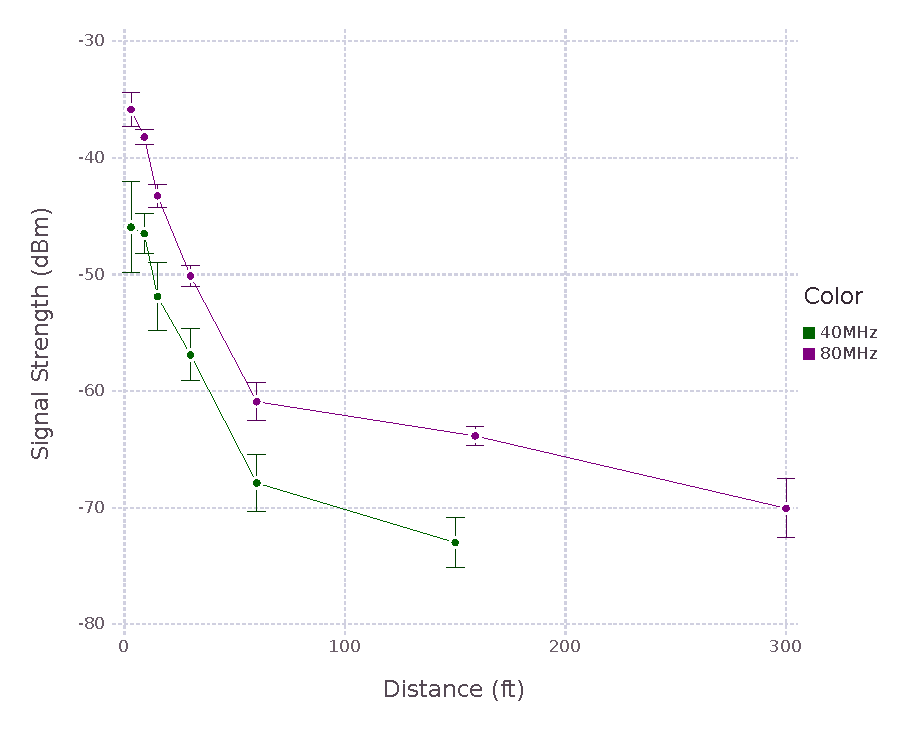
\includegraphics[width=0.5\textwidth]{figures/Intel_Outside_Beamformed}
\caption{Intel Outside Signal Strength Over Distance}
\label{fig:inteloutsidesignal}
\end{figure}

\begin{figure}[!h]
\centering
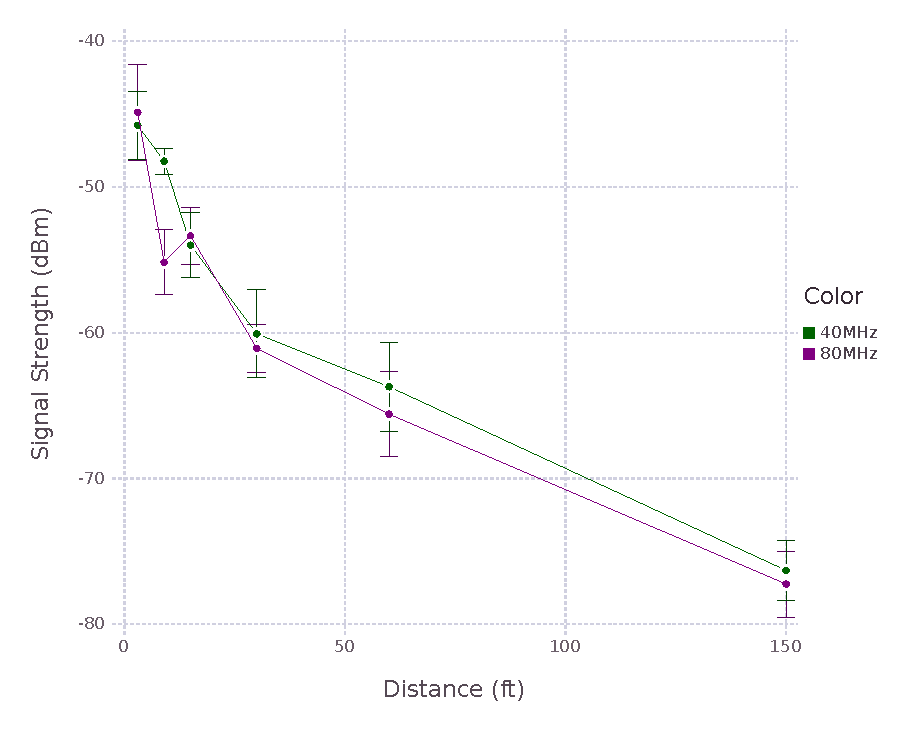
\includegraphics[width=0.5\textwidth]{figures/Mac_Outside_Beamformed}
\caption{Macbook Outside Signal Strength Over Distance}
\label{fig:macoutsidesignal}
\end{figure}


Figure~\ref{fig:inteloutsidesignal} is a perfect example of expected
behavior. As we move away from the WAP, signal strength decreases by
the square of the distance, and since dBm is a logrithmic scale, we
obtain a log-like drop-off! As expected, 80MHz outperforms 40MHz in
all cases, and even manages to maintain a connection over longer
distances.

Somewhat inexplicibly (a common theme in the collected data) the
Macbook (Figure \ref{fig:macoutsidesignal}) had a similar dropoff, but
40MHz consistently outperformed 80MHz! Given the variance shown
however, it is hard to draw any specific conclusions. \todo{this test
  was at the same time as the other...}

\subsubsection{Indoor Noisy Testing}


\begin{figure}[!h]
\centering
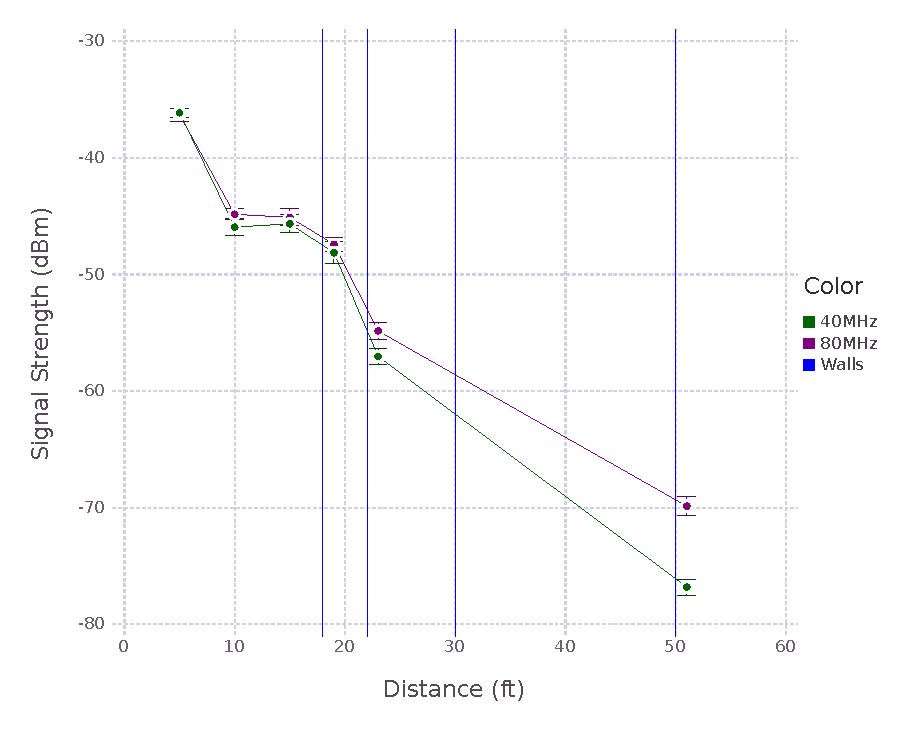
\includegraphics[width=0.5\textwidth]{figures/Intel_Inside_Beamformed}
\caption{Intel Indoor Signal Strength Over Distance}
\label{fig:intelinsidesignal}
\end{figure}

\begin{figure}[!h]
\centering
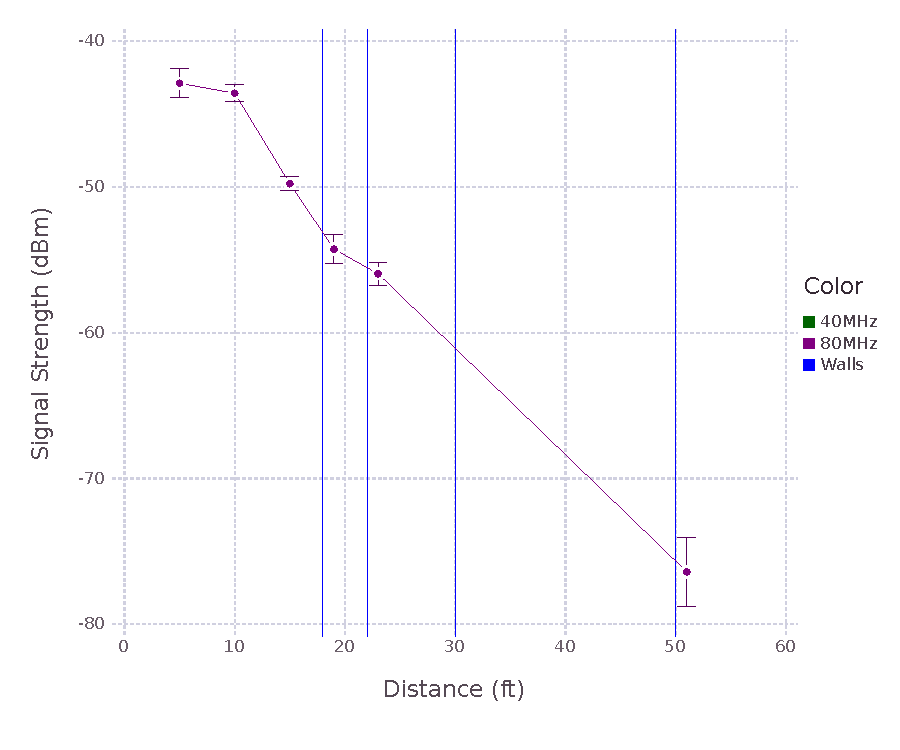
\includegraphics[width=0.5\textwidth]{figures/Mac_Inside_Beamformed}
\caption{mac Indoor Signal Strength Over Distance}
\label{fig:macinsidesignal}
\end{figure}

Indoor signal strength does, as expected, drop off significantly
faster than outdoor testing. Figure~\ref{fig:intelinsidesignal} shows
(along with approximate wall locations) the signal strength the Intel
7260 recieved in our office testing. The similar strengths seen betwen
10 and 15 ft is explained by slightly better line-of-sight in the 15ft
case over the 10ft testing location. Figure~\ref{fig:macinsidesignal}
shows the same maps for the Macbook. Unfortunately the radiotap
headers for the Macbook are inconsistently filled out, so these are
very rough estimates.




\subsection{Beamforming}


Ideally, we would compare a full non-beamformed conversation to a
beamformed one here. Unfortunately, we were unable to disuade our
client devices from advertising beamformee capabilities, and with
stock firmware the WAP cannot have beamformer capabilities disabled.
This means that while we can compare the recieved signal strength for
beamformed packets vs non-beamformed packets, this is likely to be
biased \emph{against} beamforming looking good. If the WAP decides to
not beamform consistently, it is likely that there is a channel
condition making beamforming tough. \todo{show fig with percentage
  over time?}  Thus, we have Figure~\ref{fig:intelindoorbeamresult}
which would appear to indicate that beamforming \emph{halves} the
incoming power rather than the predicted doubling. Obviously this is
not likely to be a realistic effect of beamforming, and thus an
intentionally non-beamformed test would need to be run and
compared. Outdoor data looks more plasuible, even if we still only
have a few non-beamformed
packets. Figure~\ref{fig:inteloutdoorbeambenefit} shows the benefits
over distance for locations with a non-zero number of non-beamformed
packets.
\begin{figure}[!h]
\centering
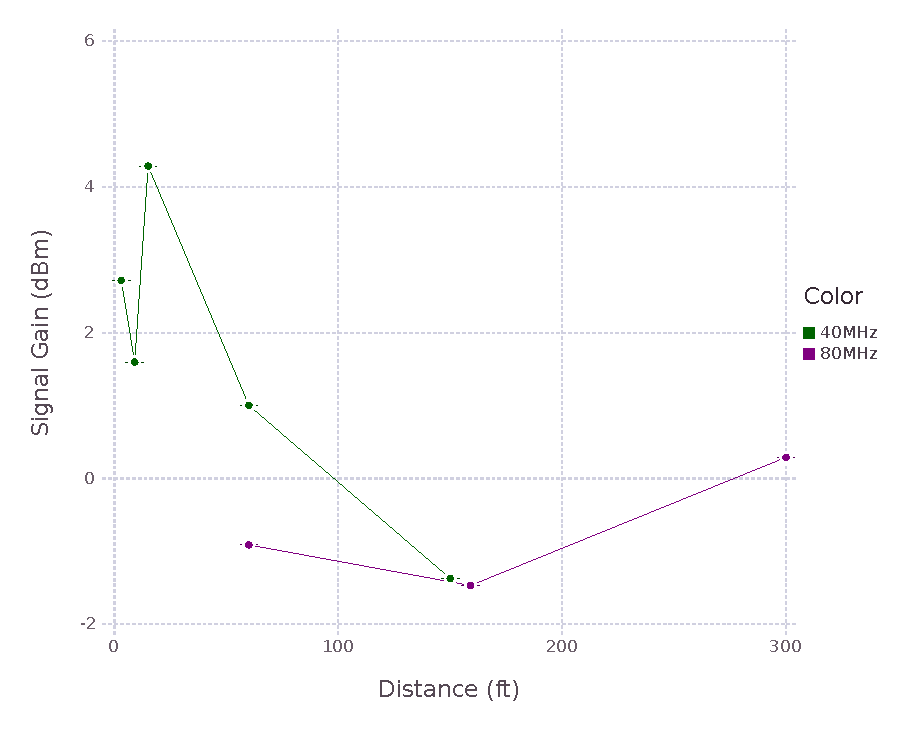
\includegraphics[width=0.5\textwidth]{figures/Intel_Outside_Beamforming_Benefit}
\caption{Intel Outdoor Beamforming Benefit}
\label{fig:inteloutdoorbeambenefit}
\end{figure}

\begin{figure}[h!]
\centering
\begin{tabular}{| c | c |}
\hline
40MHz at 51' & 80MHz at 51'\\ \hline
-2.76 dBm &  -0.31 dBm\\ \hline
\end{tabular}
\caption{Intel 7260 Indoor Beamforming Benefit}
\label{fig:intelindoorbeamresult}
\end{figure}

\begin{figure}[b!]
\centering
\begin{tabular}{| c | c || c | c | c | c | c | c |}
\hline
Chip & MHz & 5ft & 10ft & 15ft & 19ft & 23ft & 51ft\\ \hline
Intel & 40 & 0.999 & 1.0 & 0.999 & 1.0 & 0.999 & 0.655\\ \hline
Intel & 80 & 0.999 & 1.0 & 1.0 & 1.0 & 0.999 & 0.964\\ \hline
\end{tabular}
\caption{Indoor Fraction of Packets Beamformed}
\label{fig:indoorbeampercent}
\end{figure}


\begin{figure}[b!]
\centering
\begin{tabular}{| c | c || c | c | c | c | c | c | c | c |}
\hline
Chip & MHz & 3ft & 9ft & 15ft & 30ft & 60ft & 150ft & 300ft\\ \hline
Intel & 40 & 0.988 & 0.999 & 0.968 & 1.0 & 0.983 & 0.539 & na\\ \hline
Intel & 80 & 1.0 & 1.0 & 1.0 & 1.0 & 0.999 & 0.999 & 0.954\\ \hline
Mac & 40 & 0.046 & 0.042 & 0.017 & 0.006 & 0.055 & 0.140 & na\\ \hline
Mac & 80 & 0.081 & 0.062 & 0.055 & 0.033 & 0.048 & 0.105 & na\\ \hline
\end{tabular}
\caption{Outdoor Fraction of Packets Beamformed}
\label{fig:outdoorbeampercent}
\end{figure}


While still relatively untrustworthy, our outdoor beamforming benefit
measurements are much more in line with expectation. As shown in
Figures~\ref{fig:indoorbeampercent} and \ref{fig:outdoorbeampercent}
the Intel 7260 receives beamformed packets the vast majority of the
time. While it appears the Macbook does not receive many beamformed
packets, we believe that the radiotap headers it reports are
inaccurate. For example, only 1 of 8 packets have a signal strength
filled out, and many will be randomly missing other values. Thus, it
is probable that even though it explicitly reports recording
beamforming status on every packet, its reports cannot be
trusted. They are omitted from indoor testing since they are even less
plausible there.


\subsection{TCP Throughput}
While not incredibly meaningful alone, we did record TCP throughput
for all our tests. See the discussion section for our best analysis of
what occured.

Figure~\ref{fig:insidethru} shows indoor throughput, and
Figure~\ref{fig:outsidethru} shows outdoor throughput.

\begin{figure}[!h]
\centering
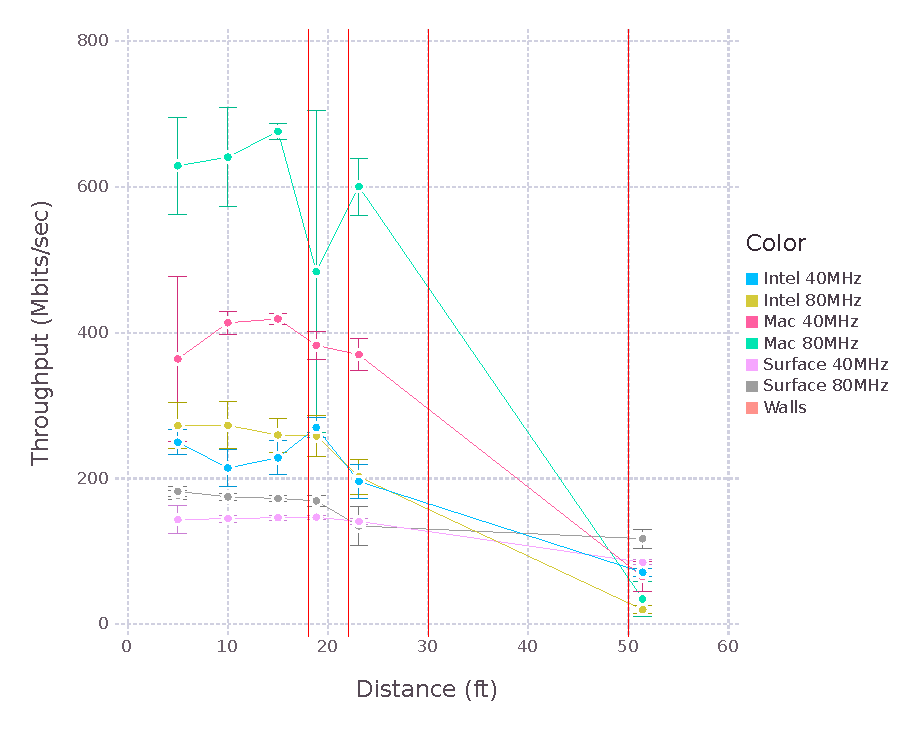
\includegraphics[width=0.5\textwidth]{figures/allchip_Inside_TCP_Throughput}
\caption{TCP Indoor Throughput}
\label{fig:insidethru}
\end{figure}

\begin{figure}[!h]
\centering
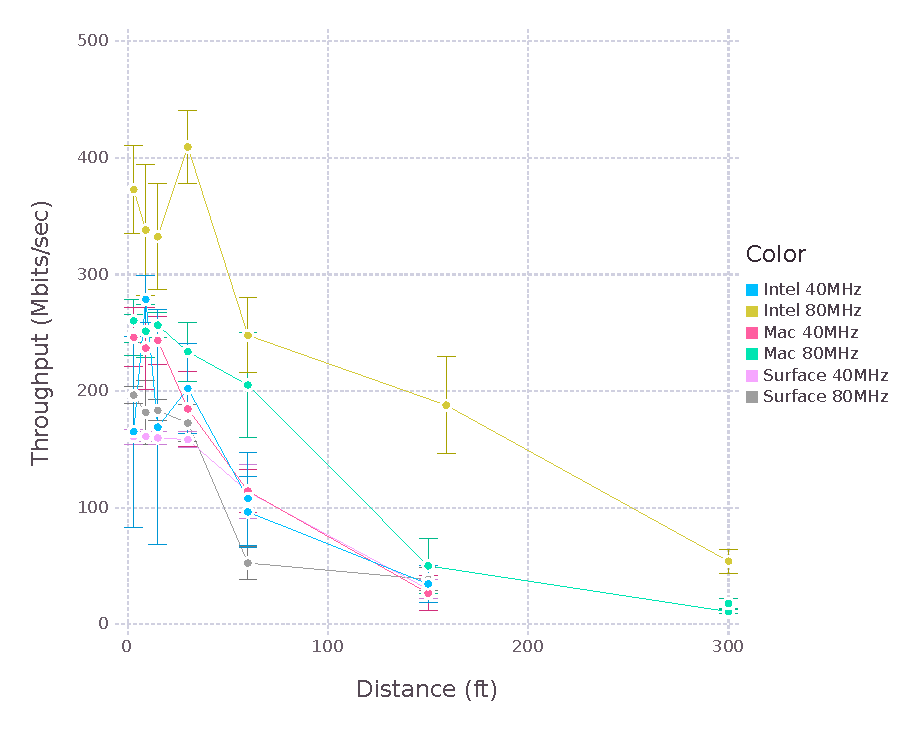
\includegraphics[width=0.5\textwidth]{figures/allchip_Outside_TCP_Throughput}
\caption{TCP Outdoor Throughput}
\label{fig:outsidethru}
\end{figure}

\subsection{MCS}
For indoors we have shown the time bucketed most common
MCS during capture by location. Figure~\ref{fig:imcs40time} and
\ref{fig:imcs40time} show the most common MCS each second for all
indoor distances. As can be seen, 40MHz has a far more stable MCS
selection, while 80MHz at mid ranges tends to switch rapidly.
\begin{figure}[!h]
\centering
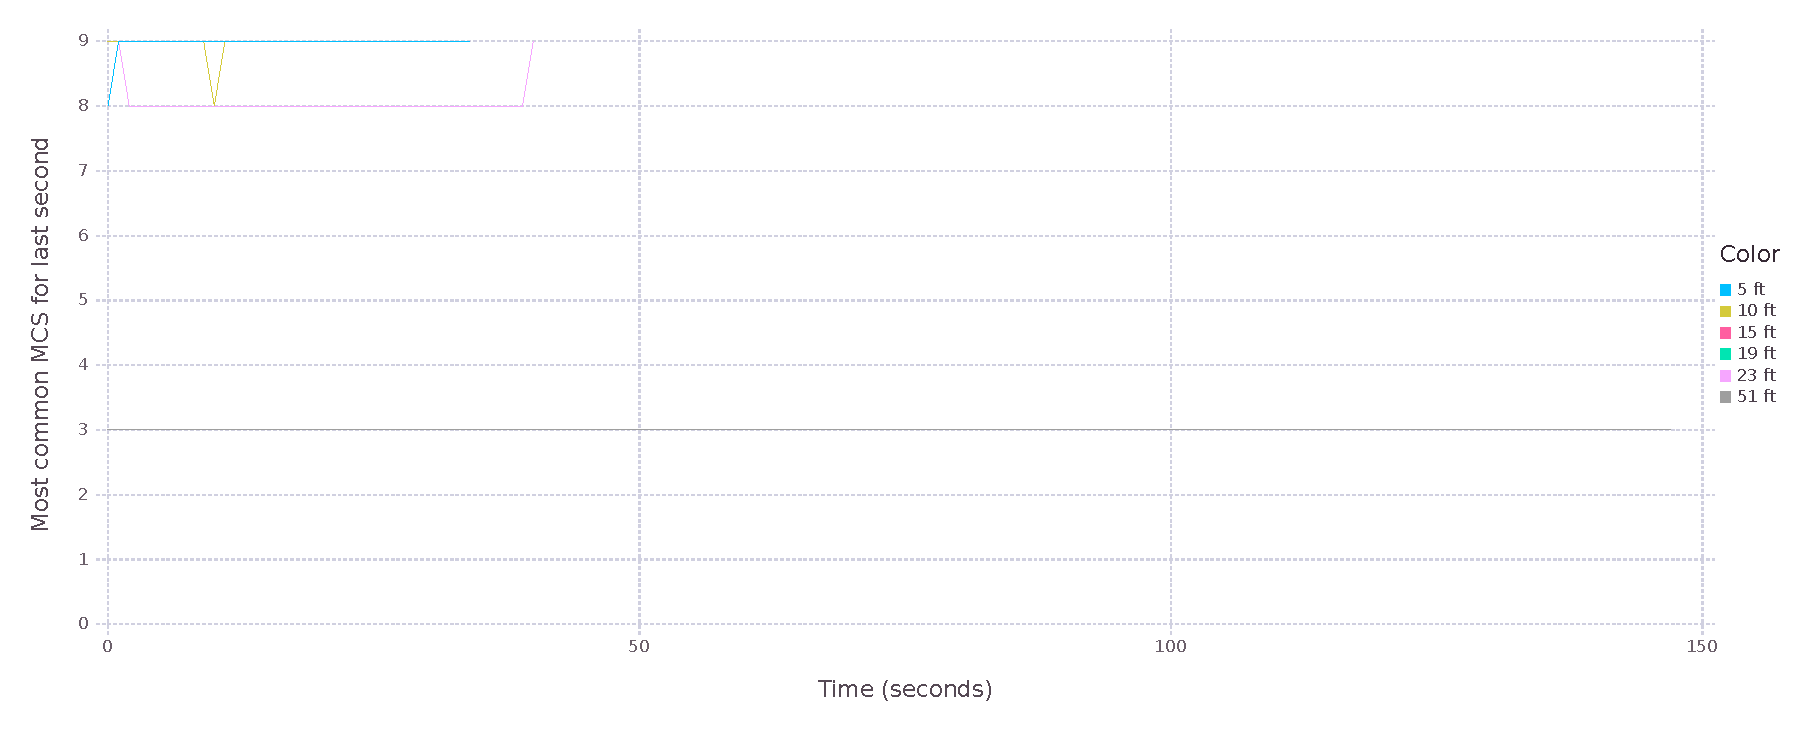
\includegraphics[width=0.5\textwidth]{figures/Intel_Inside_40_MCS}
\caption{Most Common MCS per Second Indoors for Intel at 40MHz}
\label{fig:imcs40time}
\end{figure}

\begin{figure}[!h]
\centering
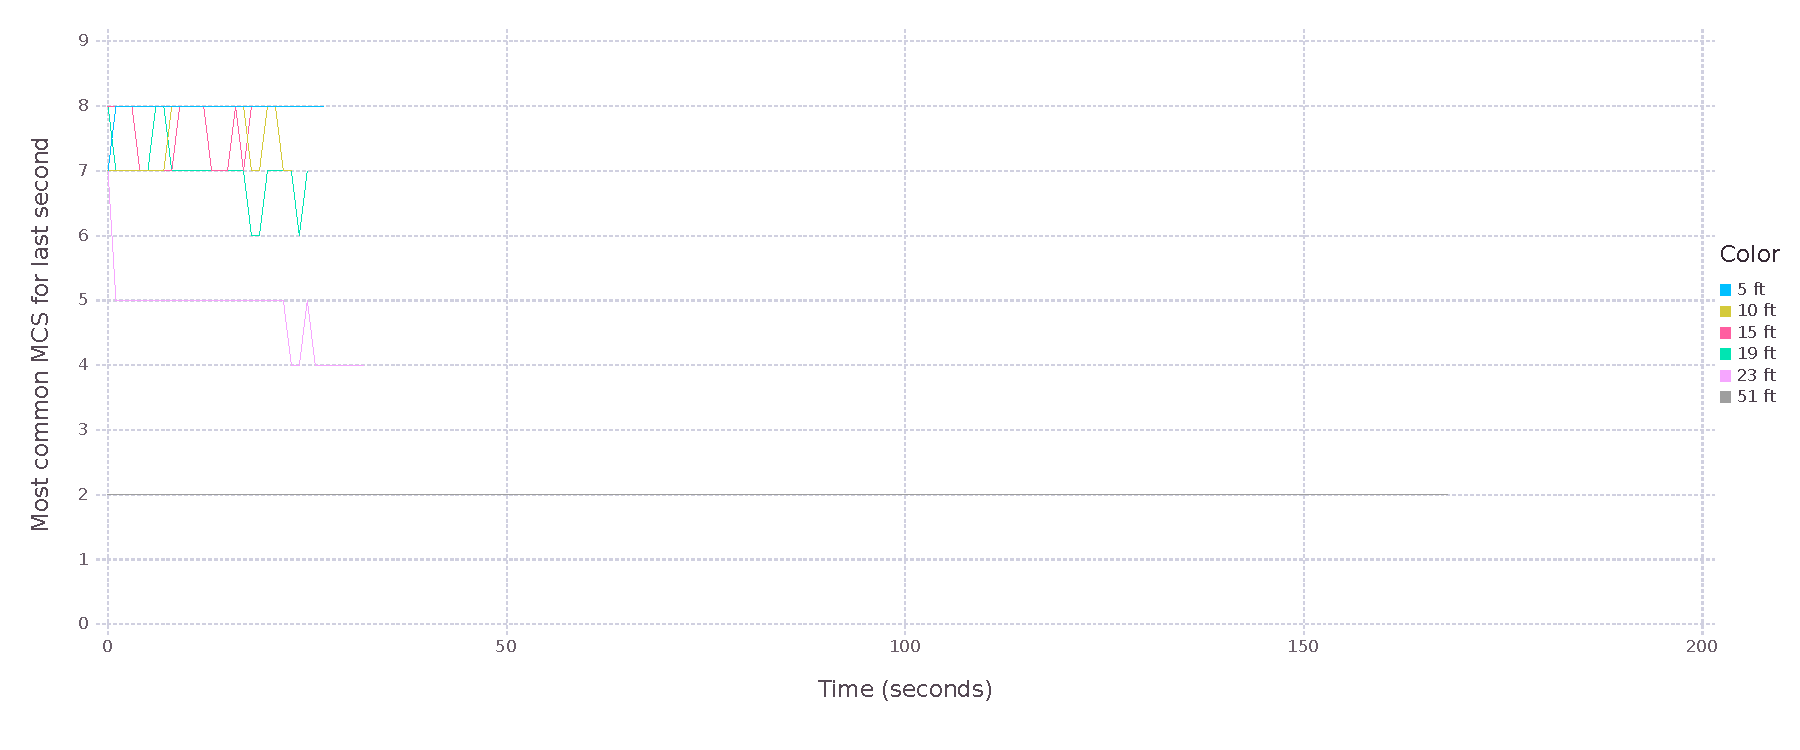
\includegraphics[width=0.5\textwidth]{figures/Intel_Inside_80_MCS}
\caption{Most Common MCS per Second Indoors for Intel at 40MHz}
\label{fig:imcs80time}
\end{figure}
